
\documentclass{llncs}

\usepackage[english]{babel}
\usepackage[utf8]{inputenc}
\usepackage{url}
\usepackage{amsmath,amssymb}
\usepackage{graphicx}
\usepackage{float}%figure environment
\usepackage[table,xcdraw]{xcolor}
%\usepackage{todonotes}
\usepackage[disable]{todonotes}
\usepackage{booktabs}
\usepackage{wrapfig}
\usepackage{multirow}
\usepackage{tikz}
\usetikzlibrary{positioning}
%\usepackage{endnotes}
\usepackage[ruled,vlined]{algorithm2e}
\usepackage{caption}
\usepackage{comment}
%\usepackage{times}
\usepackage{microtype}
\begin{document}

\title{Hybrid Question Answering with HAWK}
\author{
Ricardo Usbeck\inst{1} \and 
Ivan Ermilov\inst{1} \and
Axel-Cyrille Ngonga Ngomo\inst{1}
}

\institute{
University of Leipzig, Germany\\\email{\{usbeck,iermilov,ngonga\}@informatik.uni-leipzig.de}
}

\maketitle

\begin{abstract}
Hybrid question answering systems bridge between the Web of Data and the Document Web to answer user queries in natural language. In this demo, we present one of the first system of this type: HAWK -- Hybrid Question Answering over Linked Data. With the interface presented in the demo, we enable end users not only to use HAWK and get answers to questions but also to provide feedback to each of the processing steps of the system. By providing such feedback, the users can ensure that their answers are understood correctly and that the answer returned fulfils their information need.   
%delving deep into internal structures of a QA system
%feedback for ensemble learning 

\end{abstract}


\section{Introduction}
\todo{@Axel: Shall we write somewhere, what we are going to showcase exactly at the demo booth?}
The growing amount of information in both the Document Web and the Data Web demands innovative and easy ways to access this large amount of data. One approach to address this challenge is the provision of hybrid question answering systems, which can combine information from the Data Web and the Document Web to answer user questions. %\footnote{\url{http://greententacle.techfak.uni-bielefeld.de/~cunger/qald/}}
In this demo, we present a web-based user interface for such a framework for hybrid question answering (HQA) dubbed HAWK~\cite{HAWK_2015} which can be found at \url{http://hawk.aksw.org}.
Our demo allows laymen as well as developers to issue hybrid questions against HAWK but also to see all intermediary results of the system. Therewith, we enable (1) developers to gain valuable insights into the underlying mechanisms of the system and (2)  users to provide detailed feedback pertaining to the the intermediary results of the system. This information will be used to increase the performance of the HQA by means of active learning as well as to learn user information needs. 
In the rest of the paper, we present the aspects of the system which will be presented during the demo.  %is structured as follows: Section~\ref{sec:interaction} explains the interaction possibilities. We discuss its implications and conclude in Section~\ref{sec:conclusion}.
More information on HAWK can be found on the project webpage at \url{http://aksw.org/Projects/HAWK.html}.
\todo{@ivan hawk.aksw.org needs to point to the project page and hawk-demo.aksw.org may point to the demo to stick to the url scheme I established sofar}


\section{HAWK Interface}
\label{sec:interaction}

HAWK's dynamic pipeline will be described in detail hereafter. Our current deployment is carried out on DBpedia (structured data) and DBpedia abstracts (textual data).
As a running example, we will use the question \texttt{"Which anti-apartheid activist was born in Mvezo?"}.
For generating the answer, HAWK has to retrieve all \texttt{anti-apartheid activist} from its full-text corpus based on Wikipedia abstracts and then join this knowledge with the birth places of the persons from DBpedia Linked Data.
%To answer this, HAWK needs to fetch all \textit{anti-apartheid activist} from its full-text corpus based on Wikipedia abstract and then join this knowledge with the birth places of the persons from DBpedia Linked Data.

\paragraph{\textbf{1. Input Slit and Answer Box}:}
As means of input, HAWK provides the well-known input slit together with a dropdown menu of example queries as a main input for user queries.
%HAWK emphasizes the well-known input slit together with a dropdown menu of example queries to invite users to enter there information need. 
Results are shown on top (i.e., before the single pipeline output) in an answer box which contains (if possible) a thumbnail picture, an URI to DBpedia as well as an abstract for the particular entity, see Figure~\ref{fig:1_input}.

\begin{figure}[htb!]
\centering
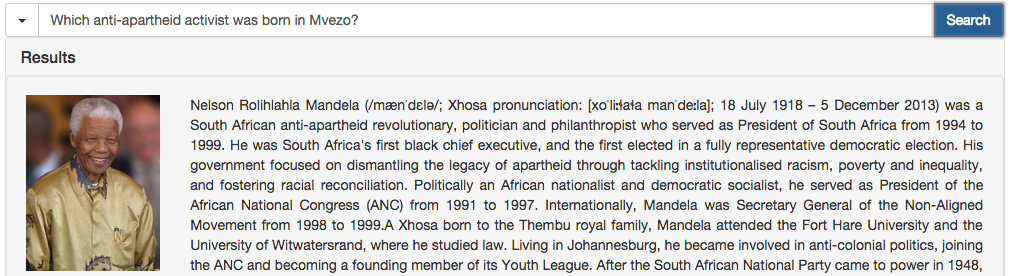
\includegraphics[width=\linewidth]{1_input}
\caption{Search slit with example dropdown menu and answer box.}
\label{fig:1_input}
\end{figure}

\paragraph{\textbf{2. Semantic Annotation}:} 
%First, 
HAWK identifies named entities from the DBpedia~\cite{jl_2014/swj_dbpedia} knowledge base.
To tackle this task, our demo application sends requests to FOX~\cite{FOX}---a federated knowledge extraction framework based on Ensemble Learning---but is also capable of using any named entity annotation service.
Currently, the demo assumes English input questions and thus tokenizes the input based on white spaces.
Afterwards, HAWK annotates each token with its part-of-speech tag (POS tag) which is used later to identify possible semantic annotations~\cite{choi2011getting}. 
Next, HAWK identifies noun phrases, i.e., semantically meaningful word groups not yet recognized by the entity annotation system. %, using the result of the POS tagging step. 
%Input tokens will be combined following manually-crafted linguistic heuristics derived from the benchmark questions. 
The results of each of the steps above can be marked by a user as correct or wrong (see Figure~\ref{fig:2_semantic_annotation}). This feedback is saved for further improvement of the  system. 

\begin{figure}[htb!]
\centering
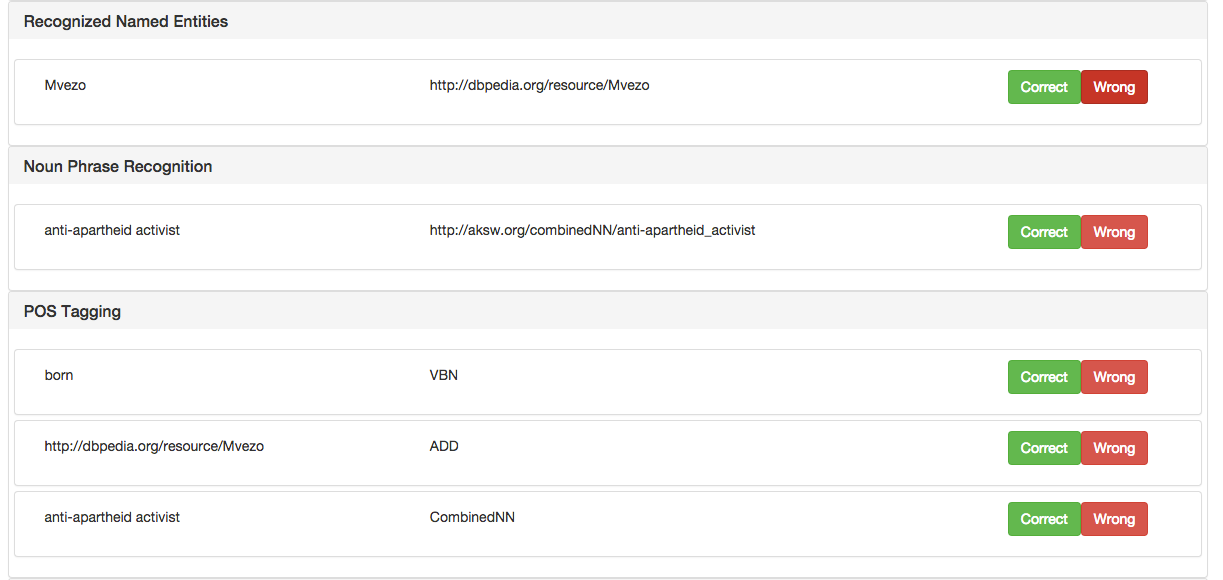
\includegraphics[width=\linewidth]{2_semantic_annotation}
\caption{Three steps of the HAWK pipeline for semantic annotation.}
\label{fig:2_semantic_annotation}
\end{figure}

\paragraph{\textbf{3. Structure Recognition}:}
%Then, 
HAWK parses the query using dependency parsing and semantic role labeling~\cite{choi2011getting}.
Therewith, HAWK recognizes the semantic dependencies between the single tokens.
The system then prunes semantically irrelevant parts of the tree to avoid the injection of noise in the next process steps based on manually defined rules.
The resulting tree structure contains only semantically relevant (combined) token and entities, i.e., individuals from the underlying knowledge base. 
HAWK then tries to map the tokens that were not yet mapped to a knowledge base to properties and classes from the underlying ontology. To this end, it uses  a fuzzy string search.
The trees as well as the semantically annotated nodes for our running example are depicted in Figure~\ref{fig:3_structure_recognition}.
\begin{figure}[htb!]
\centering
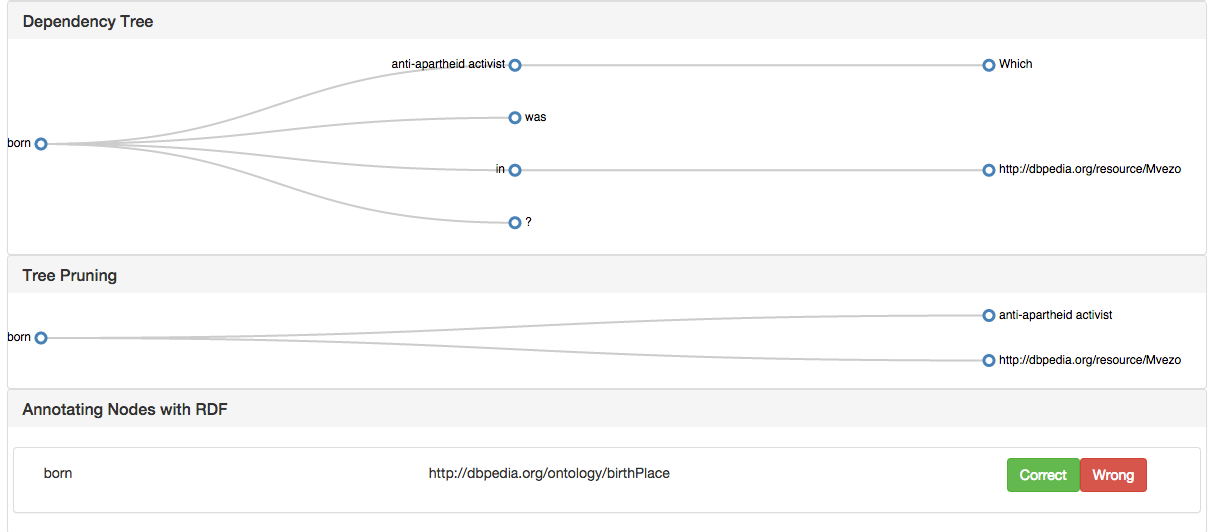
\includegraphics[width=\linewidth]{3_structure_recognition}
\caption{Full and pruned predicate argument trees as well as semantically annotated nodes.}
\label{fig:3_structure_recognition}
\end{figure}

\paragraph{\textbf{4. Generating Hybrid SPARQL Queries}:}
Finally, HAWK generates hybrid SPARQL queries from the extracted multitude of semantic information.
The HQA system uses the Apache Jena FUSEKI\footnote{\url{http://jena.apache.org/documentation/serving_data/}} server, which implements a full-text search predicate which maps textual information to a certain individual URI from a target knowledge.

In short, for each combination of semantic annotated nodes in the pruned tree, HAWK generates a hybrid SPARQL query using several full-text search techniques, e.g., fuzzy-search or exact match.
This results in covering every possible SPARQL graph pattern for a given input question as well as in a large number of SPARQL queries to test and rank ( i.e., up to 15.000 per input question from the QALD 5 benchmark\footnote{\url{http://greententacle.techfak.uni-bielefeld.de/~cunger/qald/index.php?x=home&q=5}}).
To reduce the number of queries sent to the server, HAWK applies more than a dozen pruning pruning heuristics such as discarding unconnected query graphs or query that do not abide by the ontology.

The final step of the pipeline is to rank the remaining set of SPARQL query answer sets. 
Currently, we apply overlap-based ranking in the demo.
It is based on the intuition that the same result set can be generated by several hybrid SPARQL queries and thus, counts the resulting answer sets based on a bucketing process.
We show the final SPARQL query for our running example in Figure~\ref{fig:4_final_SPARQL}.

\begin{figure}[htb!]
\centering
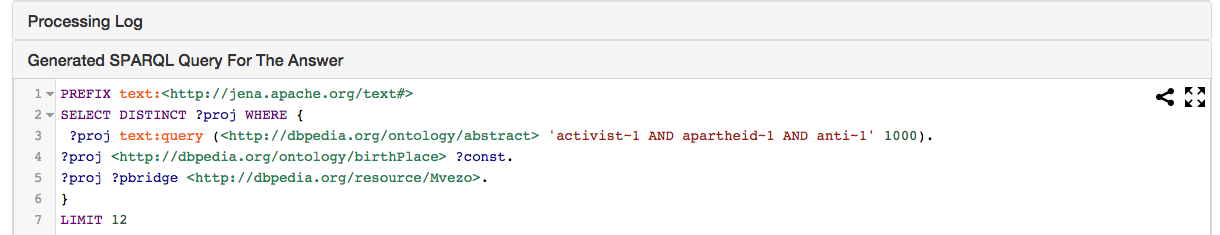
\includegraphics[width=\linewidth]{4_final_sparql}
\caption{Boxes for process log and top-1 ranked SPARQL query.}
\label{fig:4_final_SPARQL}
\end{figure}


%More detailed descriptions of each step of HAWK's pipeline are available at~\cite{HAWK_2015}.
%Moreover, HAWK's modular architecture allows to exchange single modules in the pipeline to account.


%\section{Evaluation}
%\label{sec:discussion}
%Dataset           & \multicolumn{1}{l}{Optimal Ranking} & \multicolumn{1}{l}{Feature-based Ranking} & \multicolumn{1}{l}{Overlap-based Ranking} \\ \midrule
%QALD-5 - training & 0.30 (15 out of 26)                 & 0.06 (22 out of 26)                       & 0.08 (22 out of 26)                       \\
%Taken from ASSESS
%\subsection{Evaluation of the user interface}
%Moreover, we performed a system usability study (SUS)\footnote{\url{http://www.measuringu.com/sus.php}} to validate the design of our web-interface. 
%7 users -  with a good or no knowledge of natural language processing, language generation or e-learning - answered our survey resulting in a SUS-Score of 85.3. This score assign the mark $S$ to the current interface of ASSESS and places it into the 10\% best category of interface, meaning that users of the interface are likely to recommend it to a friend. In particular, all users found that they did not need to learn anything to use the tool and that the interface was intuitive. Figure~\ref{fig:sus-assess} shows the average voting per question and its standard deviation. In particular, all users consistently do not think that they need the support of a technical person to be able to use this system (Q4) nor need to learn a lot of things before they could get going with this system (Q10).

\section{Conclusion}
\label{sec:conclusion}
In this paper, we described the web-based interface of HAWK which enables to delve deep into the single steps of the HAWK pipeline and, most importantly, allows to give feedback on how well these steps address the users' information needs. 
In the future, we will use the feedback provided by the users to learn how to interpret user queries  as well as to enable the user to manipulate the HQA pipeline directly. 
%\vspace{.2cm}

\textbf{Acknowledgments}
This work has been supported by the FP7 project GeoKnow (GA No. 318159), the BMWI project SAKE and the EuroStars project DIESEL.

\bibliographystyle{abbrv}
\bibliography{llncs}

\end{document}